% RCSID: "$Id: NimVerT.tex,v 1.1 2018/03/30 20:22:12 penton Exp $"

\begin{deluxetable}{llccc|llccc|llccc}
\tablecaption{\tacq{IMAGE} Co-alignment Measurements\label{tab:coaligned}}
\tablecolumns{15}
\tabcolsep 2pt
\tabletypesize{\tiny}
\tablehead{
\colhead{\textit{PROPOSID}} & \colhead{\textit{ROOT}} & \colhead{Configuration\tablenotemark{a}} & \colhead{\textit{ACQSLEW}} & \colhead{\textit{APER}} &
\colhead{PID} & \colhead{\textit{ROOT}} & \colhead{Config\tablenotemark{a}} & \colhead{\textit{ACQSLEW}} & \colhead{APER} &
\colhead{PID} & \colhead{\textit{ROOT}} & \colhead{Config\tablenotemark{a,c}} & \colhead{\textit{ACQSLEW}} & \colhead{APER} \\
\colhead{(PID)} & \colhead{\textit{NAME}} & \colhead{\#1} & \colhead{[\textit{X},\textit{Y}] (\arcsec)} & \colhead{\textit{YPOS}} &
\colhead{} & \colhead{\textit{NAME}} & \colhead{\#2} & \colhead{[\textit{X},\textit{Y}] (\arcsec)} & \colhead{\textit{YPOS}} &
\colhead{} & \colhead{\textit{NAME}} & \colhead{\#1} & \colhead{[\textit{X},\textit{Y}] (\arcsec)} & \colhead{\textit{YPOS}} \\
\colhead{(1)} & \colhead{(2)} & \colhead{(3)}& \colhead{(4)} & \colhead{(5)} &
\colhead{(6)} & \colhead{(7)} &\colhead{(8)} & \colhead{(9)} & \colhead{(10)} &
\colhead{(11)} & \colhead{(12)} & \colhead{(13)} & \colhead{(14)} & \colhead{(15)}

}
\startdata
\toprule
\multicolumn{15}{c}{C21}\tablenotemark{b}\\
\midrule
\pid{13616} & lci4a2e3q & PSA$\times$MIRA & [ 0.001, 0.133] & 127.1 &\pid{13616} & lci4a2e5q & PSA$\times$MIRB & [ 0.016, 0.027] & 127.1 & \dots & \dots & \dots & \dots & \dots  \\
\pid{13526} & lcgq03dbq & PSA$\times$MIRA & [ 0.166,-0.168] & 127.1 &\pid{13526} & lcgq03dlq & PSA$\times$MIRB & [-0.029, 0.006] & 127.1 &\pid{13526} & lcgq03dtq & PSA$\times$MIRA & [0.032,-0.026] & 127.1 \\
\pid{13526} & lcgq01q5q & PSA$\times$MIRB & [-0.888, 0.298] & 127.1 &\pid{13526} & lcgq01qdq & BOA$\times$MIRA & [-0.038, 0.013] & 126.1 &\pid{13526} & lcgq01qjq & PSA$\times$MIRB & [0.027,-0.078] & 126.1 \\
\pid{13526} & lcgq02hmq & BOA$\times$MIRA & [ 0.058, 0.305] & 127.1 &\pid{13526} & lcgq02huq & BOA$\times$MIRB & [-0.015,-0.105] & 126.1 &\pid{13526} & lcgq02i0q & BOA$\times$MIRA & [0.006, 0.063] & 126.1 \\
\midrule
\multicolumn{15}{c}{C22}\\
\midrule
\pid{14035} & lcsla2bhq & PSA$\times$MIRA & [-0.020, 0.105] & 125.1 &\pid{14035} & lcsla2bjq & PSA$\times$MIRB & [ 0.022, 0.007] & 125.1 & \dots & \dots & \dots & \dots & \dots \\
\pid{13972} & lcri01fzq & PSA$\times$MIRB & [ 0.189,-0.273] & 125.1 &\pid{13972} & lcri01g7q & BOA$\times$MIRA & [-0.011, 0.109] & 126.1 &\pid{13972} & lcri01geq & PSA$\times$MIRB & [ 0.036,-0.092] & 126.1 \\
\pid{13972} & lcri02h8q & BOA$\times$MIRA & [ 0.201,-0.315] & 125.1 &\pid{13972} & lcri02hgq & BOA$\times$MIRB & [ 0.026, 0.010] & 126.1 &\pid{13972} & lcri02hmq & BOA$\times$MIRA & [-0.018, 0.038] & 126.1 \\
\midrule
\multicolumn{15}{c}{C23}\\
\midrule
\pid{14452} & ld3la2ojq & PSA$\times$MIRA & [-0.017, 0.075] & 125.1 &\pid{14452} & ld3la2onq & PSA$\times$MIRB & [-0.002, 0.021] & 125.1 & \dots & \dots & \dots & \dots & \dots \\
\pid{14440} & ld3701gtq & PSA$\times$MIRB & [-0.104, 0.088] & 125.1 &\pid{14440} & ld3701h1q & BOA$\times$MIRA & [-0.018, 0.105] & 126.1 &\pid{14440} & ld3701h7q & PSA$\times$MIRB & [ 0.016,-0.071] & 126.1 \\
\pid{14440} & ld3702mzq & BOA$\times$MIRA & [ 0.390, 0.322] & 125.1 &\pid{14440} & ld3702n9q & BOA$\times$MIRB & [ 0.001, 0.030] & 126.1 &\pid{14440} & ld3702nhq & BOA$\times$MIRA & [-0.012, 0.057] & 126.1 \\
\midrule
\multicolumn{15}{c}{C24}\\
\midrule
\pid{14857} & ldozpbf5q & PSA$\times$MIRA & [-0.058,-0.355] & 125.1 &\pid{14857} & ldozpbfbq & PSA$\times$MIRB & [ 0.020, 0.023] & 125.1 &\pid{14857} & ldozpbfhq & PSA$\times$MIRA & [-0.020,-0.011] & 125.1 \\
\pid{14857} & ldozbadhq & PSA$\times$MIRB & [-0.366,-0.967] & 125.1 &\pid{14857} & ldozbadpq & BOA$\times$MIRA & [-0.013, 0.113] & 126.1 &\pid{14857} & ldozbadvq & PSA$\times$MIRB & [ 0.029,-0.059] & 126.1 \\
\pid{14857} & ldozbbleq & BOA$\times$MIRA & [ 0.290, 0.114] & 125.1 &\pid{14857} & ldozbblmq & BOA$\times$MIRB & [ 0.006,-0.011] & 126.1 &\pid{14857} & ldozbblsq & BOA$\times$MIRA & [-0.015, 0.060] & 126.1 \\
\bottomrule
\enddata
\tablenotetext{a}{Each row tests the co-alignment of two \tacq{IMAGE} configurations. The first ``Configuration\#1'' exposure centers the target, then the ``Configuration\#2'' exposure measures the co-alignment.
A second Configuration\#1 \tacq{IMAGE} provides a second co-alignment measurement of the BOA configuration \#2s.}
\tablenotetext{b}{During C21, both the FGS-to-SI (\pid{13636}) and TA monitoring program (\pid{13526}) executed PSA$\times$MIRA and PSA$\times$MIRB back-to-back \tacq{IMAGE}s.
\tablenotetext{c}{``\dots'' indicate that there is no confirming PSA$\times$MIRA Configuration\#1 exposure.}
\pid{13526} contained an additional PSA$\times$MIRA exposure as part of the MIRB re-enablement effort. Both programs provided consistent results, but the more complete \pid{13526} dataset is used in the analysis of this ISR. }
\tablecomments{FGS-to-SI alignment programs (\pid{13616}, \pid{14035}, \& \pid{14452}) contain a singe pair of \tacq{IMAGE}s, while the COS TA programs contain a third Configuration\#1 \tacq{IMAGE}. }
\end{deluxetable}


\begin{deluxetable}{llccccc}
\tablecaption{Initial \tacq{IMAGE} Co-alignment Measurements\label{tab:coalignedMERGE}}
\tablecolumns{7}
\tabcolsep 2pt
\tabletypesize{\footnotesize}
\tablehead{
\colhead{Configuration} & \colhead{Configuration} & \colhead{Offset\#1}  & \colhead{Offset\#2}  & \colhead{Avg Offset} & \colhead{\textit{APERYPOS} Correction} & \colhead{Est. Offset}\\
\colhead{\#1} & \colhead{\#2} & \colhead{[AD,XD] (\arcsec)} & \colhead{[AD,XD] (\arcsec)}  & \colhead{} & \colhead{[AD,XD] (\arcsec)} & \colhead{[AD,XD] (\arcsec)}\\
\colhead{(1)} & \colhead{(2)} & \colhead{(3)}& \colhead{(4)} & \colhead{(5)} & \colhead{(6)} & \colhead{(7)}
}
\startdata
\toprule
\multicolumn{7}{c}{C21}\\
\midrule
%PSA$\times$MIRA & PSA$\times$MIRB & [ 0.016, 0.027]  & \dots\tablenotetext{a}  & [ 0.016, 0.027]	& [ 0.000,0.000]	& [ 0.016, 0.027] \\
PSA$\times$MIRA & PSA$\times$MIRB & [-0.029, 0.006]  & [0.032,-0.026]  & [-0.031, 0.016]	& [ 0.000,0.000]	& [-0.031, 0.016] \\
PSA$\times$MIRB & BOA$\times$MIRA & [-0.038, 0.013]  & [0.027,-0.078]  & [-0.033, 0.046]	& [ 0.000,0.053]	& [-0.033, 0.072] \\
BOA$\times$MIRA & BOA$\times$MIRB &	[-0.015,-0.105]  & [0.006, 0.063]  & [-0.011,-0.084]	& [ 0.000,0.053]	& [-0.011,-0.058] \\
\midrule
\multicolumn{7}{c}{C22}\\
\midrule
PSA$\times$MIRA & PSA$\times$MIRB & [ 0.022, 0.007]  & \dots\tablenotemark{a}    & [ 0.022, 0.007]	& [ 0.000, 0.000]	& [ 0.022, 0.007] \\
PSA$\times$MIRB & BOA$\times$MIRA & [-0.011, 0.109]  & [ 0.036,-0.092]   & [-0.024, 0.101]	& [ 0.000,-0.053]	& [-0.024, 0.074] \\
BOA$\times$MIRA & BOA$\times$MIRB &	[ 0.026, 0.010]  & [-0.018, 0.038]   & [ 0.022,-0.014]	& [ 0.000,-0.053]	& [ 0.022,-0.040] \\
\midrule
\multicolumn{7}{c}{C23}\\
\midrule
PSA$\times$MIRA & PSA$\times$MIRB & [-0.002, 0.021]  & \dots\tablenotemark{a}    & [-0.002, 0.021]	& [ 0.000, 0.000]	& [-0.002, 0.021] \\
PSA$\times$MIRB & BOA$\times$MIRA & [-0.018, 0.105]  & [ 0.016,-0.071]   & [-0.017, 0.088]	& [ 0.000,-0.053]	& [-0.017, 0.062] \\
BOA$\times$MIRA & BOA$\times$MIRB &	[ 0.001, 0.030]  & [-0.012, 0.057]   & [ 0.007, 0.122]	& [ 0.000,-0.053]	& [ 0.007, 0.095] \\
\midrule
\multicolumn{7}{c}{C24}\\
\midrule
PSA$\times$MIRA & PSA$\times$MIRB & [ 0.020, 0.023]  & [-0.020,-0.011]   & [ 0.020, 0.017]	& [ 0.000, 0.000]	& [ 0.020, 0.017] \\
PSA$\times$MIRB & BOA$\times$MIRA & [-0.013, 0.113]  & [ 0.029,-0.059]   & [-0.021, 0.086]	& [ 0.000,-0.053]	& [-0.021, 0.060] \\
BOA$\times$MIRA & BOA$\times$MIRB &	[ 0.006,-0.011]  & [-0.015, 0.060]   & [ 0.011,-0.036]	& [ 0.000,-0.053]	& [ 0.011,-0.062] \\
\bottomrule
\enddata
\tablenotetext{a}{For C22 and C23, no confirming PSA$\times$MIRA Configuration\#1 exposures were acquired.}
\end{deluxetable}
\begin{deluxetable}{lcccccc}
\tablecolumns{7}
\tabcolsep 6pt
\tabletypesize{\footnotesize}
\tablecaption{C20--C24 \tacq{IMAGE} Co-Alignment Results\label{tab:finalcoalign}}
\tablehead{
\colhead{} & \multicolumn{2}{c}{PSA} & \multicolumn{2}{c}{BOA} & \multicolumn{2}{c}{Measurement}\\
\colhead{Base} & \colhead{$\times$MIRA} & \colhead{$\times$MIRB} & \colhead{$\times$MIRA} &\colhead{$\times$MIRB} & \multicolumn{2}{c}{Uncertainty\tablenotemark{a}}\\
\colhead{Configuration} & \colhead{[AD,XD]\arcsec} & \colhead{[AD,XD]\arcsec} & \colhead{[AD,XD]\arcsec} & \colhead{[AD,XD]\arcsec} & \colhead{(p)} & \colhead{(\arcsec)}\\
\colhead{(1)} & \colhead{(2)} & \colhead{(3)} & \colhead{(4)} & \colhead{(5)} & \colhead{(6)} & \colhead{(7)}

}
\startdata
\toprule
\multicolumn{7}{c}{C20}\\
\midrule
PSA$\times$MIRA	&			[1,1]	&	[0.019,0.009]	&	[0.007,-0.065]	&	[0.026,0.037]	&	0.850	&	0.020 \\
PSA$\times$MIRB	&	[-0.019,-0.009]	&			[1,1]	&	[-0.012,-0.074]	&	[0.007,0.028]	&	1.041	&	0.024 \\
BOA$\times$MIRA	&	[-0.007,0.065]	&	[0.012,0.074	&			[1,1]	&	[0.019,0.102]	&	1.201	&	0.028\\
BOA$\times$MIRB	&	[-0.026,-0.037]	&	[-0.007,-0.028]	&	[-0.019,-0.102]	&			[1,1]	&	1.343	&	0.032\\
\midrule
\multicolumn{7}{c}{C21}\\
\midrule
PSA$\times$MIRA	&			[1,1]	&	[0.031,-0.016]	&	[0.063,-0.088]	&	[0.074,-0.030]	&	0.850	&	0.020 \\
PSA$\times$MIRB	&	[-0.031,0.016]	&			[1,1]	&	[0.033,-0.072]	&	[0.043,-0.014]	&	1.041	&	0.024 \\
BOA$\times$MIRA	&	[-0.063,0.088]	&	[-0.033,0.072]	&	 		[1,1]	&	[0.011, 0.058]	&	1.201	&	0.028\\
BOA$\times$MIRB	&	[-0.074,0.030]	&	[-0.043,0.014]	&	[-0.011,-0.058]	&	 		[1,1]	&	1.343	&	0.032\\
\midrule
\multicolumn{7}{c}{C22}\\
\midrule
PSA$\times$MIRA	&	     [1,1 ]	&	[-0.022,-0.007]	&	[0.002,-0.081]	&	[-0.021,-0.041]	&	0.850	&	0.020\\
PSA$\times$MIRB	&	[0.022,0.007 ]	&	 		[1,1]	&	[0.024,-0.074]	&	[ 0.002,-0.034]	&	1.041	&	0.024\\
BOA$\times$MIRA	&	[-0.002,0.081]	&	[-0.024,0.074]	&	  		[1,1]	&	[-0.022,0.040]	&	1.201	&	0.028\\\
BOA$\times$MIRB	&	[0.021, 0.041]	&	[-0.002,0.034]	&	[0.022,-0.040]	&	[1,1]	&	1.343	&	0.032\\
\midrule
\multicolumn{7}{c}{C23}\\
\midrule
PSA$\times$MIRA	&	     [1,1 ]	&	[ 0.002,-0.021]	&	[0.023,-0.081]	&	[0.013,-0.019]	&	0.850	&	0.020\\
PSA$\times$MIRB	&	[-0.002,0.021]	&			[1,1 ]	&	[0.021,-0.060]	&	[0.011, 0.002]	&	1.041	&	0.024\\
BOA$\times$MIRA	&	[-0.023,0.081]	&	[-0.021, 0.060]	&	     [1,1 ]	&	[-0.011,0.062]	&	1.201	&	0.028\\\
BOA$\times$MIRB	&	[-0.013,0.019]	&	[-0.011,-0.002]	&	[0.011,-0.062]	&			[1,1 ]	&	1.343	&	0.032\\
\midrule
\multicolumn{7}{c}{C24}\\
\midrule
PSA$\times$MIRA	&	     [1,1]	&	[-0.020,-0.017]	&	[-0.003,-0.079]	&	[-0.001, -0.100]	&	0.850	&	0.020\\
PSA$\times$MIRB	&	[0.020,0.017]	&			[1,1]	&	[ 0.017,-0.062]	&	[0.019,-0.083]	&	1.041	&	0.024\\
BOA$\times$MIRA	&	[0.003,0.079]	&	[-0.017,0.062]	&			[1,1]	&	[0.002,-0.021]	&	1.201	&	0.028\\\
BOA$\times$MIRB	&	[0.001,0.100]	&	[-0.019, 0.083]	&	[-0.002, 0.021]	&	   [1,1 ]	&	1.343	&	0.032\\
\midrule
\multicolumn{7}{c}{C20--C24}\\
\midrule
PSA$\times$MIRA	&	    		[    1 ,    1]	&	[-0.002,-0.015]	&	[0.021,-0.082]	&	[0.016,-0.047]	&	0.425	&	0.010\\
PSA$\times$MIRB	&	[{\bf 0.002},{\bf 0.015}]	&			[1,1 ]	&	[0.024,-0.067]	&	[0.019,-0.032]	&	0.520	&	{\bf 0.012}\\
BOA$\times$MIRA	&	[{\bf-0.021},{\bf 0.082}]	&	[-0.024,0.067]	&	   [1,1 ]	&	[-0.005,0.035]	&	0.601	&	{\bf 0.014}\\
BOA$\times$MIRB	&	[{\bf-0.016},{\bf 0.047}]	&	[-0.019,0.032]	&	[0.005,-0.035]	&	     [1,1 ]	&	0.672	&	{\bf 0.016}\\
\bottomrule
\enddata
\tablenotetext{a}{An average of the AD and XD platescales was used to estimate the uncertainty (in \arcsec) in column 7.}
\tablecomments{To determine the co-alignment of \tacq{IMAGE} Config\#2 To Config\#1, Config\#2 is the base configuration. Use that
row at the desired column (of Config\#1) to determine the co-alignment. The alignment order is that if a Config\#1 \tacq{IMAGE} is followed by a Config\#2 \tacq{IMAGE},
one should expect the  given \textit{ACQSLEWX} and \textit{ACSLEWY}.
Final co-alignment averages, and uncertainties, over C20--24 are shown in {\bf bold}.}
\end{deluxetable}

%[ 0.016, 0.027]	& [ 0.000,0.000]	& [ 0.016, 0.027]
%[-0.033, 0.046]	& [ 0.000,0.053]	& [-0.033, 0.072]
%[-0.011,-0.084]	& [ 0.000,0.053]	& [-0.011,-0.058]
%
%[ 0.022, 0.007]	& [ 0.000, 0.000]	& [ 0.022, 0.007]
%[-0.024, 0.101]	& [ 0.000,-0.053]	& [-0.024, 0.074]
%[ 0.022,-0.014]	& [ 0.000,-0.053]	& [ 0.022,-0.040]
%
%[-0.002, 0.021]	& [ 0.000, 0.000]	& [-0.002,0.021]
%[-0.017, 0.088]	& [ 0.000,-0.053]	& [-0.017,0.062]
%[ 0.007, 0.122]	& [ 0.000,-0.053]	& [ 0.007,0.095]
%
%[ 0.020, 0.017]	& [ 0.000, 0.000]	& [ 0.020,0.017]
%[-0.021, 0.086]	& [ 0.000,-0.053]	& [-0.021,0.060]
%[ 0.011,-0.036]	& [ 0.000,-0.05]3	& [ 0.011,-0.062]

%\begin{table}
%\caption{NUV Image Analysis\label{tab:nuvimageanal}}
%\begin{tabular}{lcccr}
%\toprule
%\multirow{5}{*}{\parbox[c]{1 in}{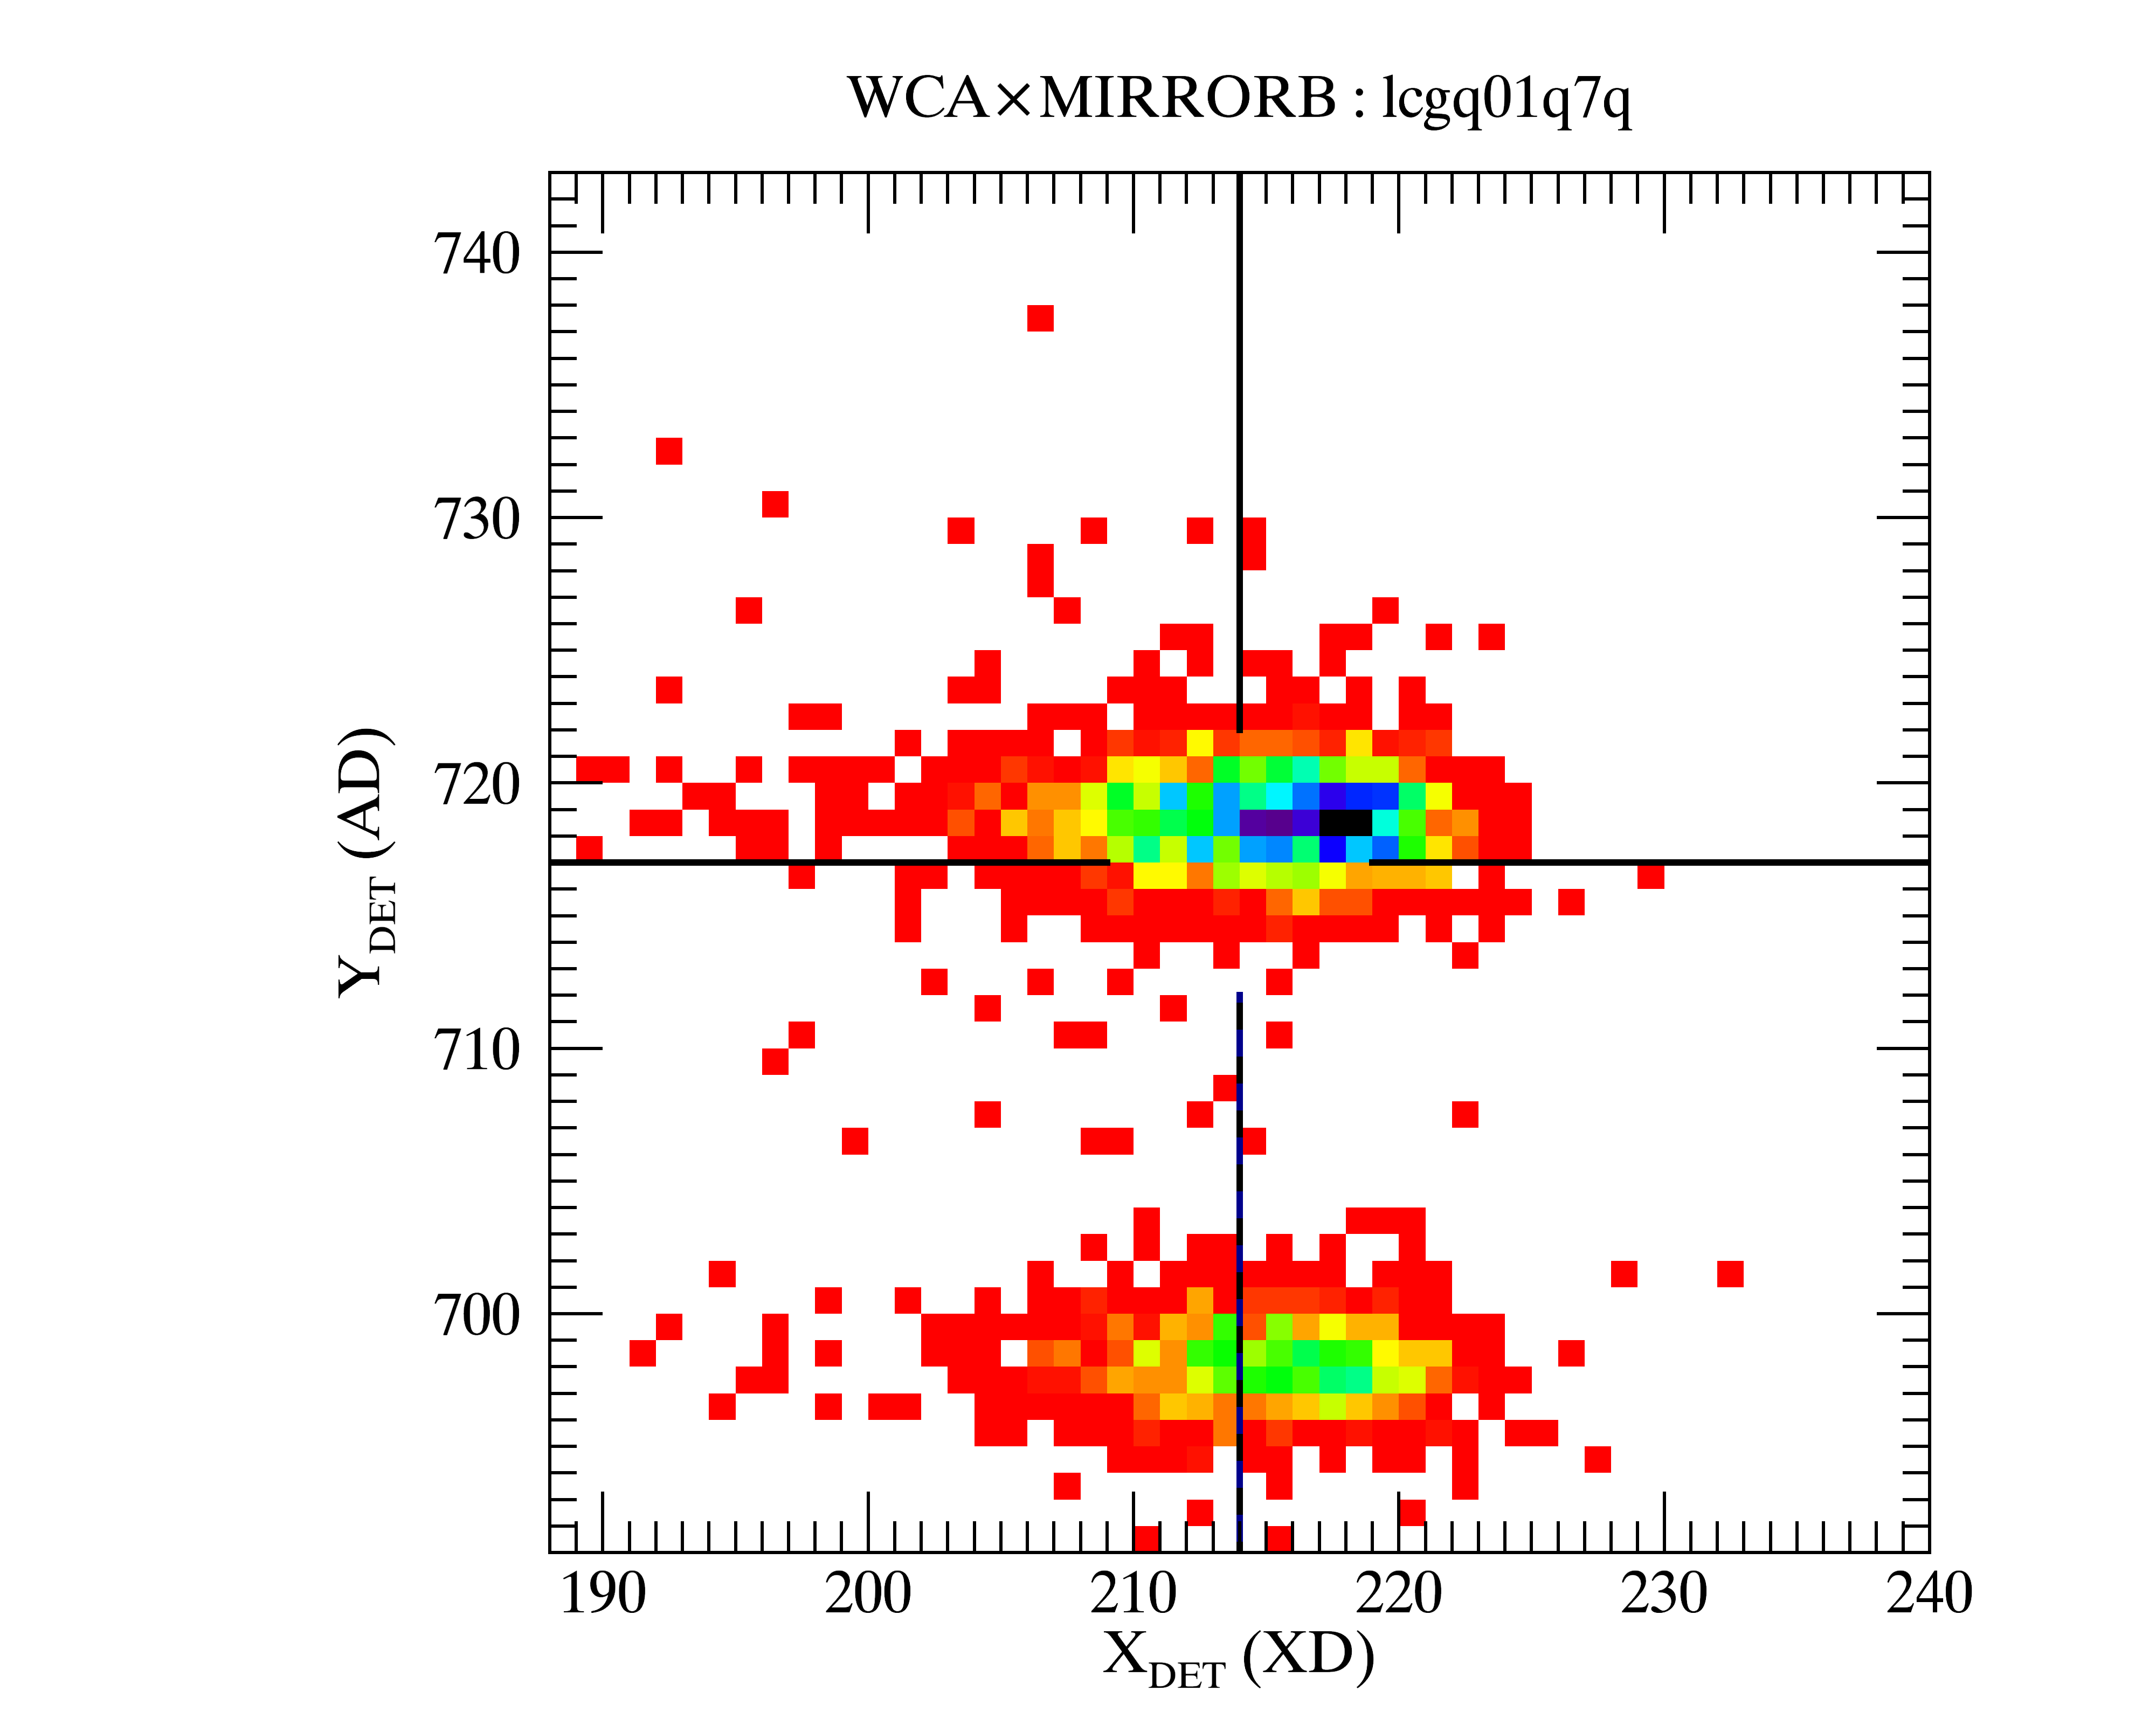
\includegraphics[width=1in]{png/lcgq01q7q_wca.png}}} & WCA &  \textit{APERTURE} &PSA & \multirow{5}{*}{\parbox[c]{1 in}{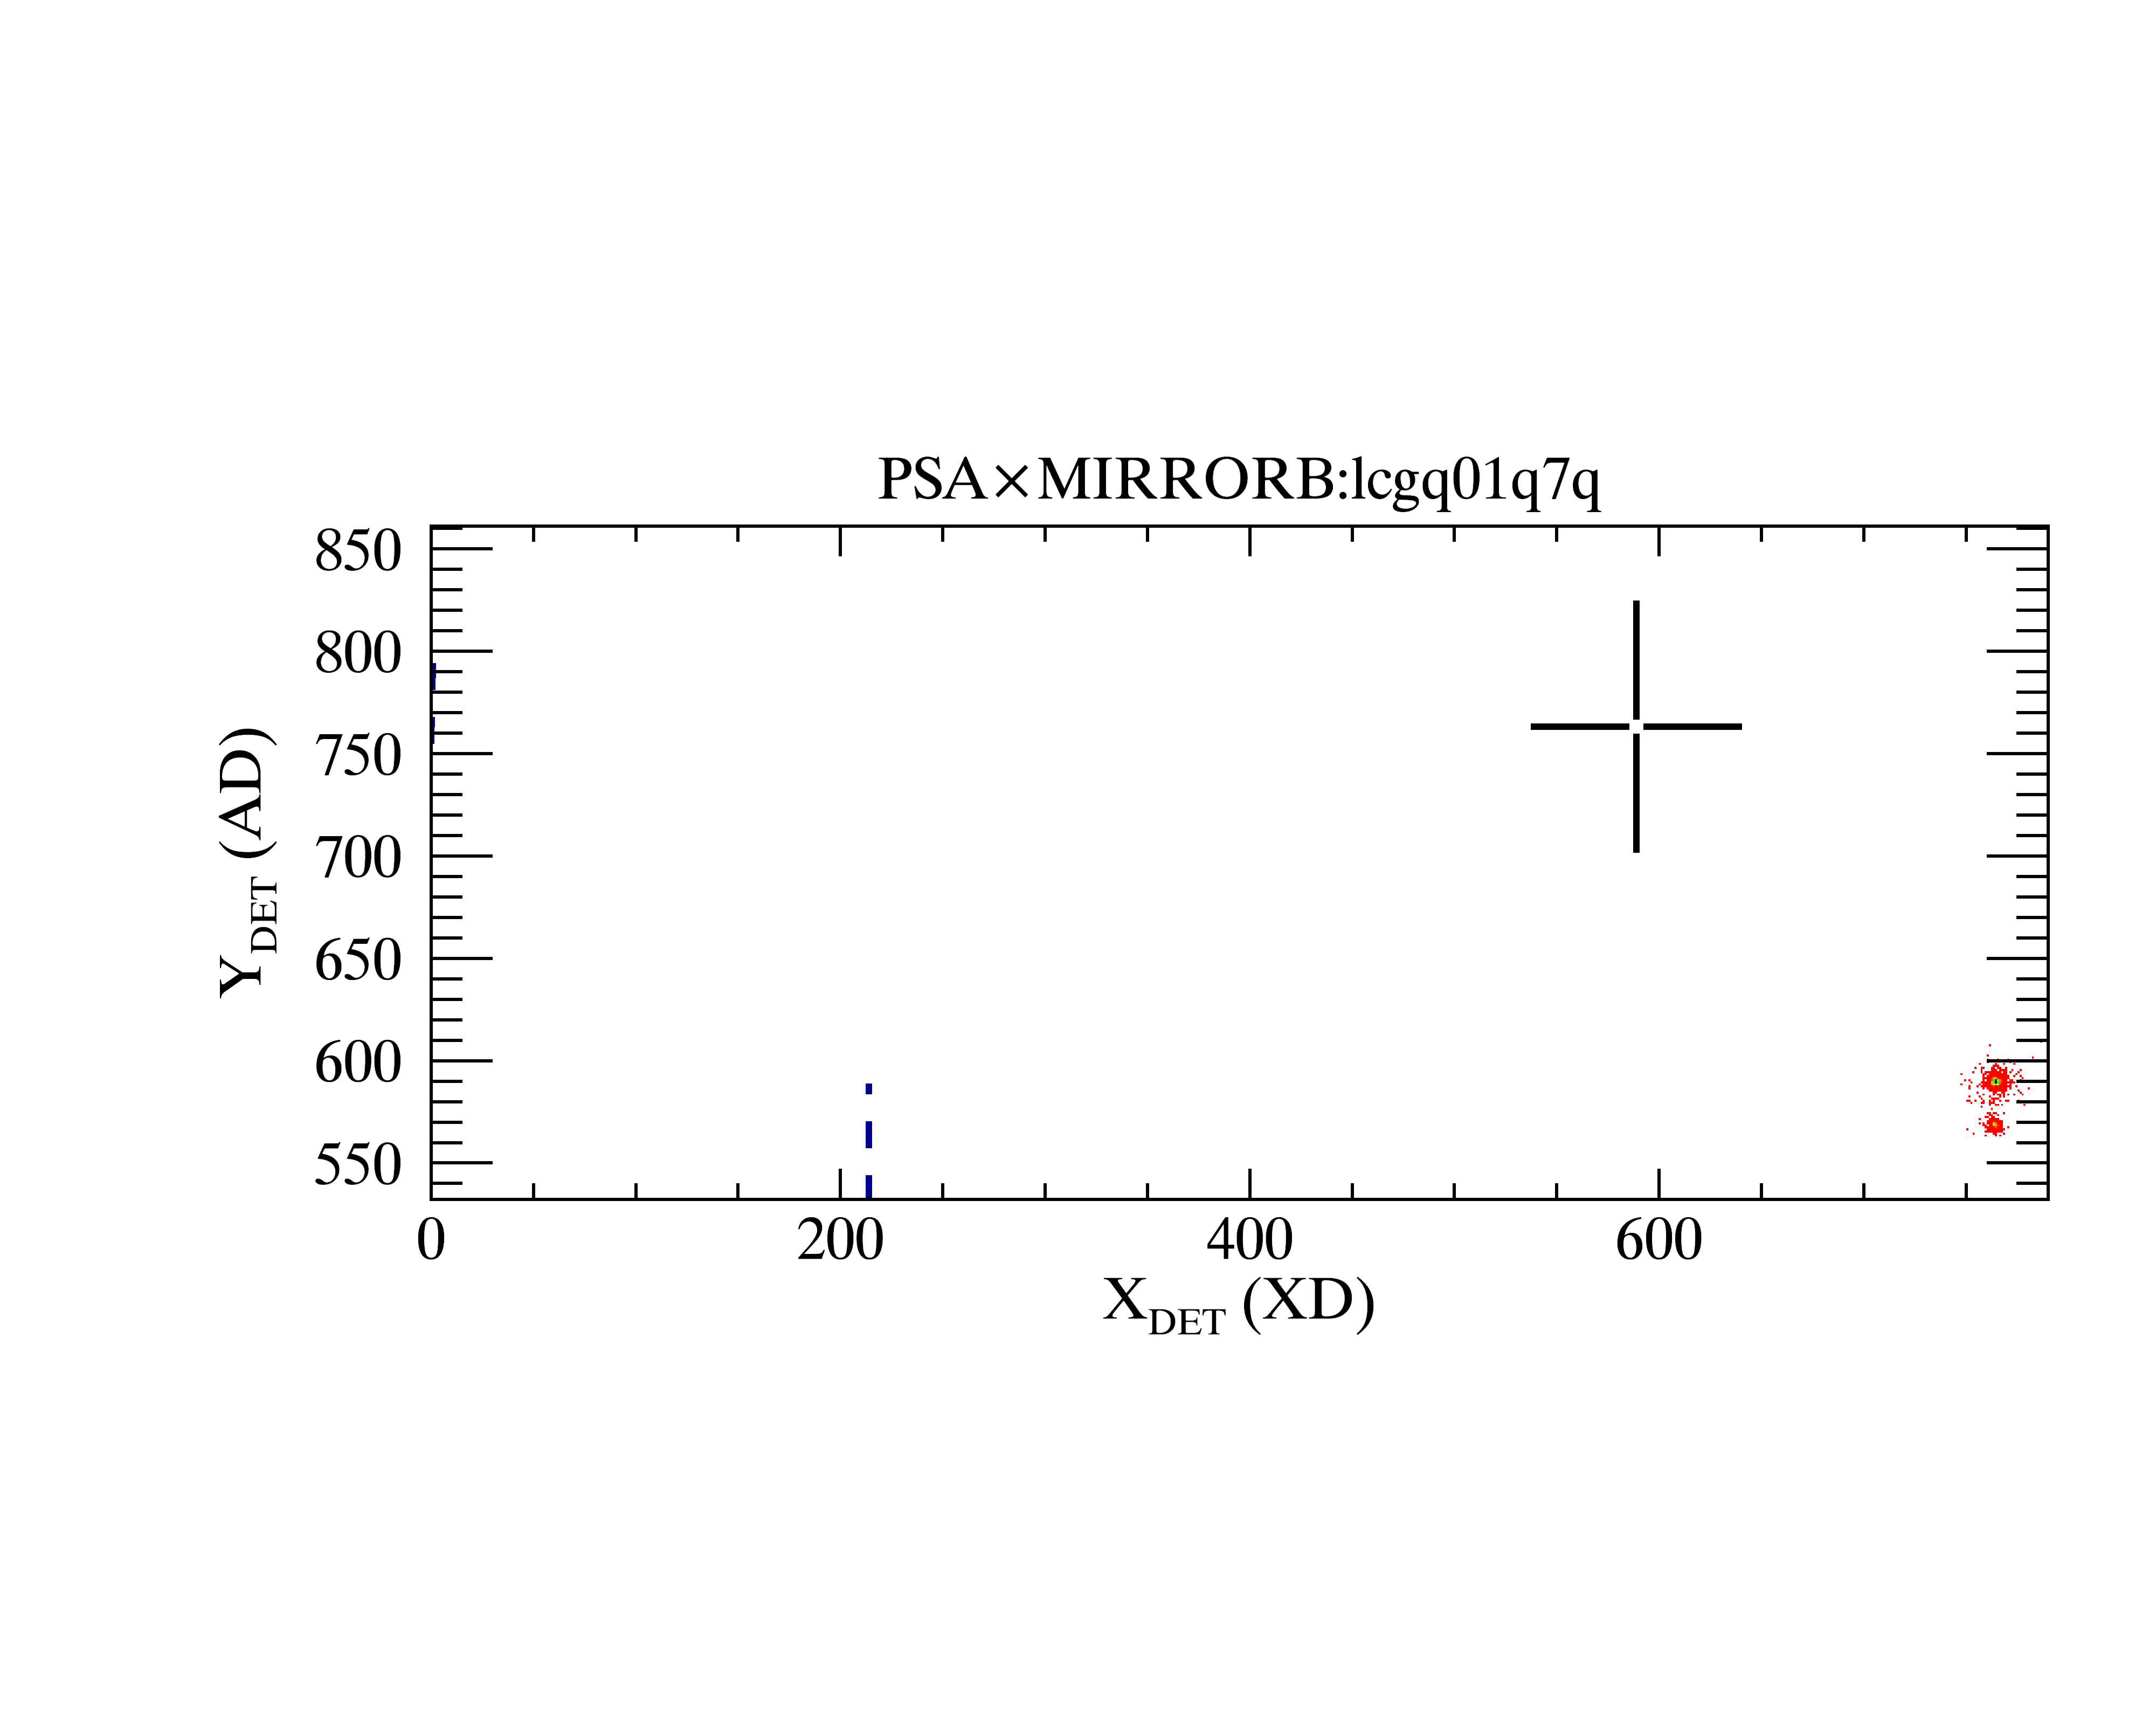
\includegraphics[width=1in]{png/lcgq01q7q_sa.png}}} \\
% &lcgq01q7q & \textit{ROOTNAME} & lcgq01q7q &  \\
% &[717.0,214.0] & [AD,XD] Standard Measurement & [763.1,588.9] &   \\
% &[717.0,214.0] & [AD,XD] Alternate Measurement & [1.0,1.0] & \\
% &[0.0,0.0] & [AD,XD] Standard - Alternate  & [762.1,587.9] & \\
%\midrule
%\multirow{5}{*}{\parbox[c]{1 in}{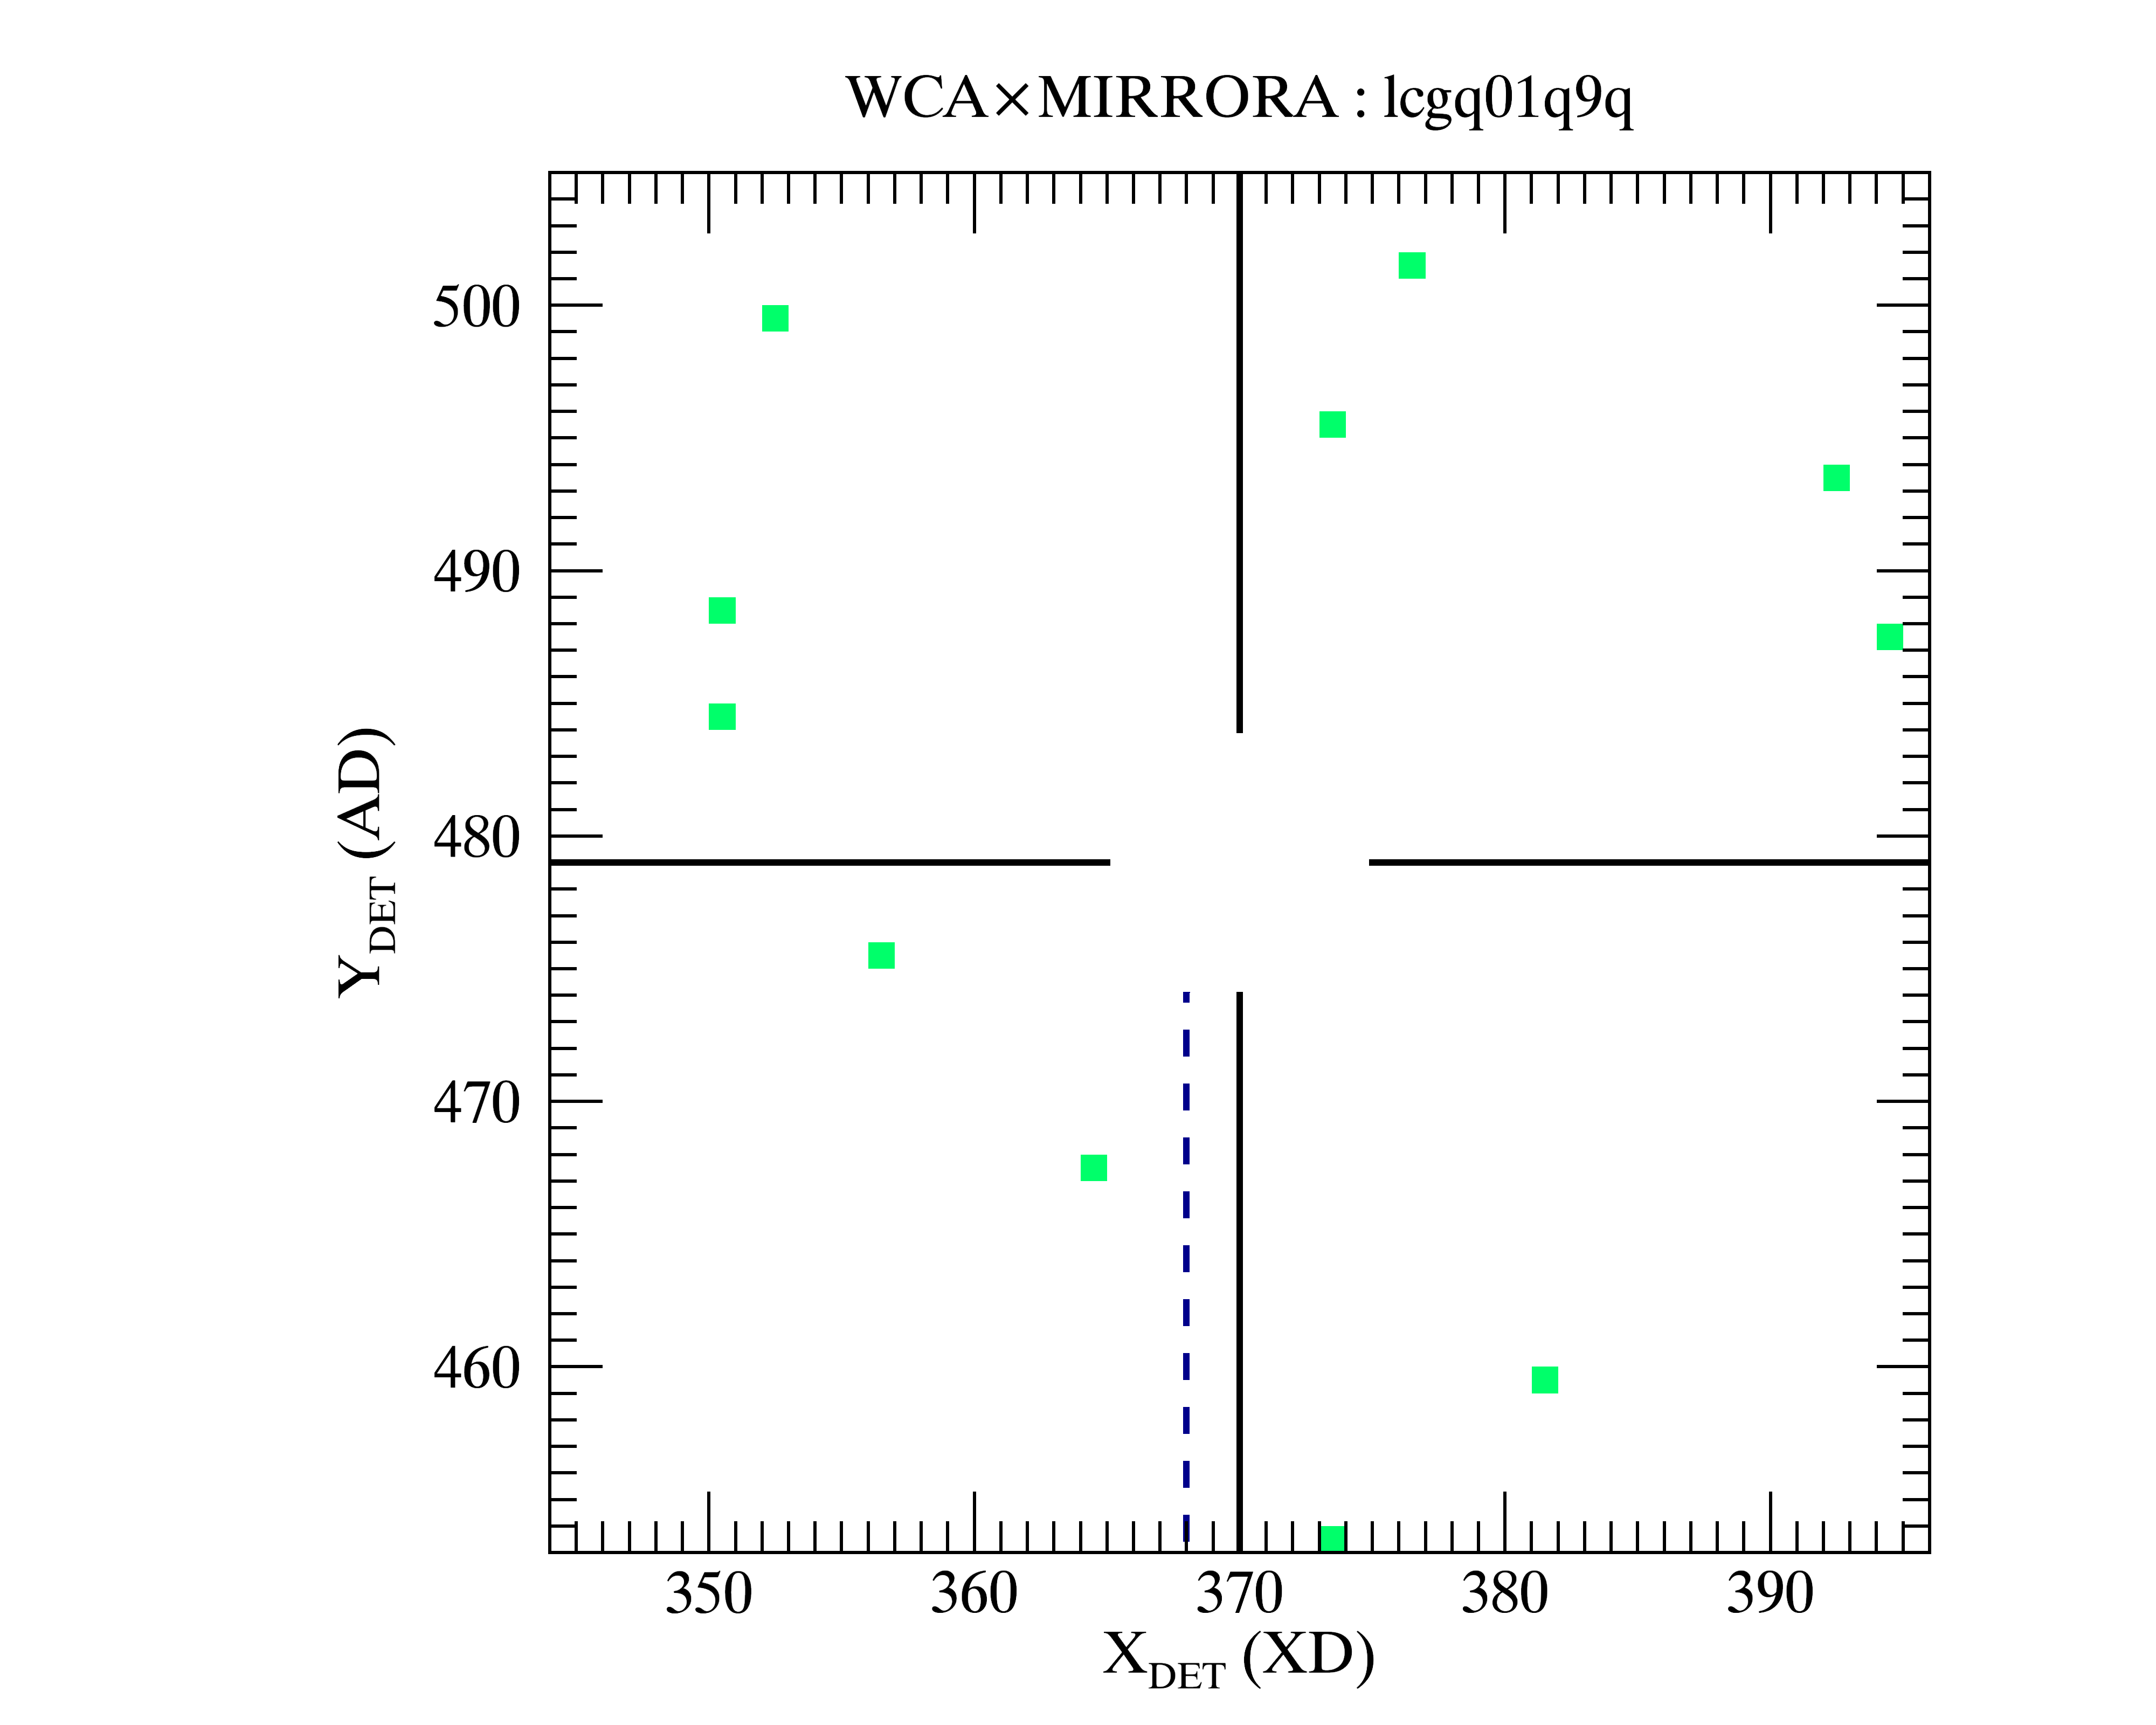
\includegraphics[width=1in]{png/lcgq01q9q_wca.png}}} & WCA &  \textit{APERTURE} &BOA & \multirow{5}{*}{\parbox[c]{1 in}{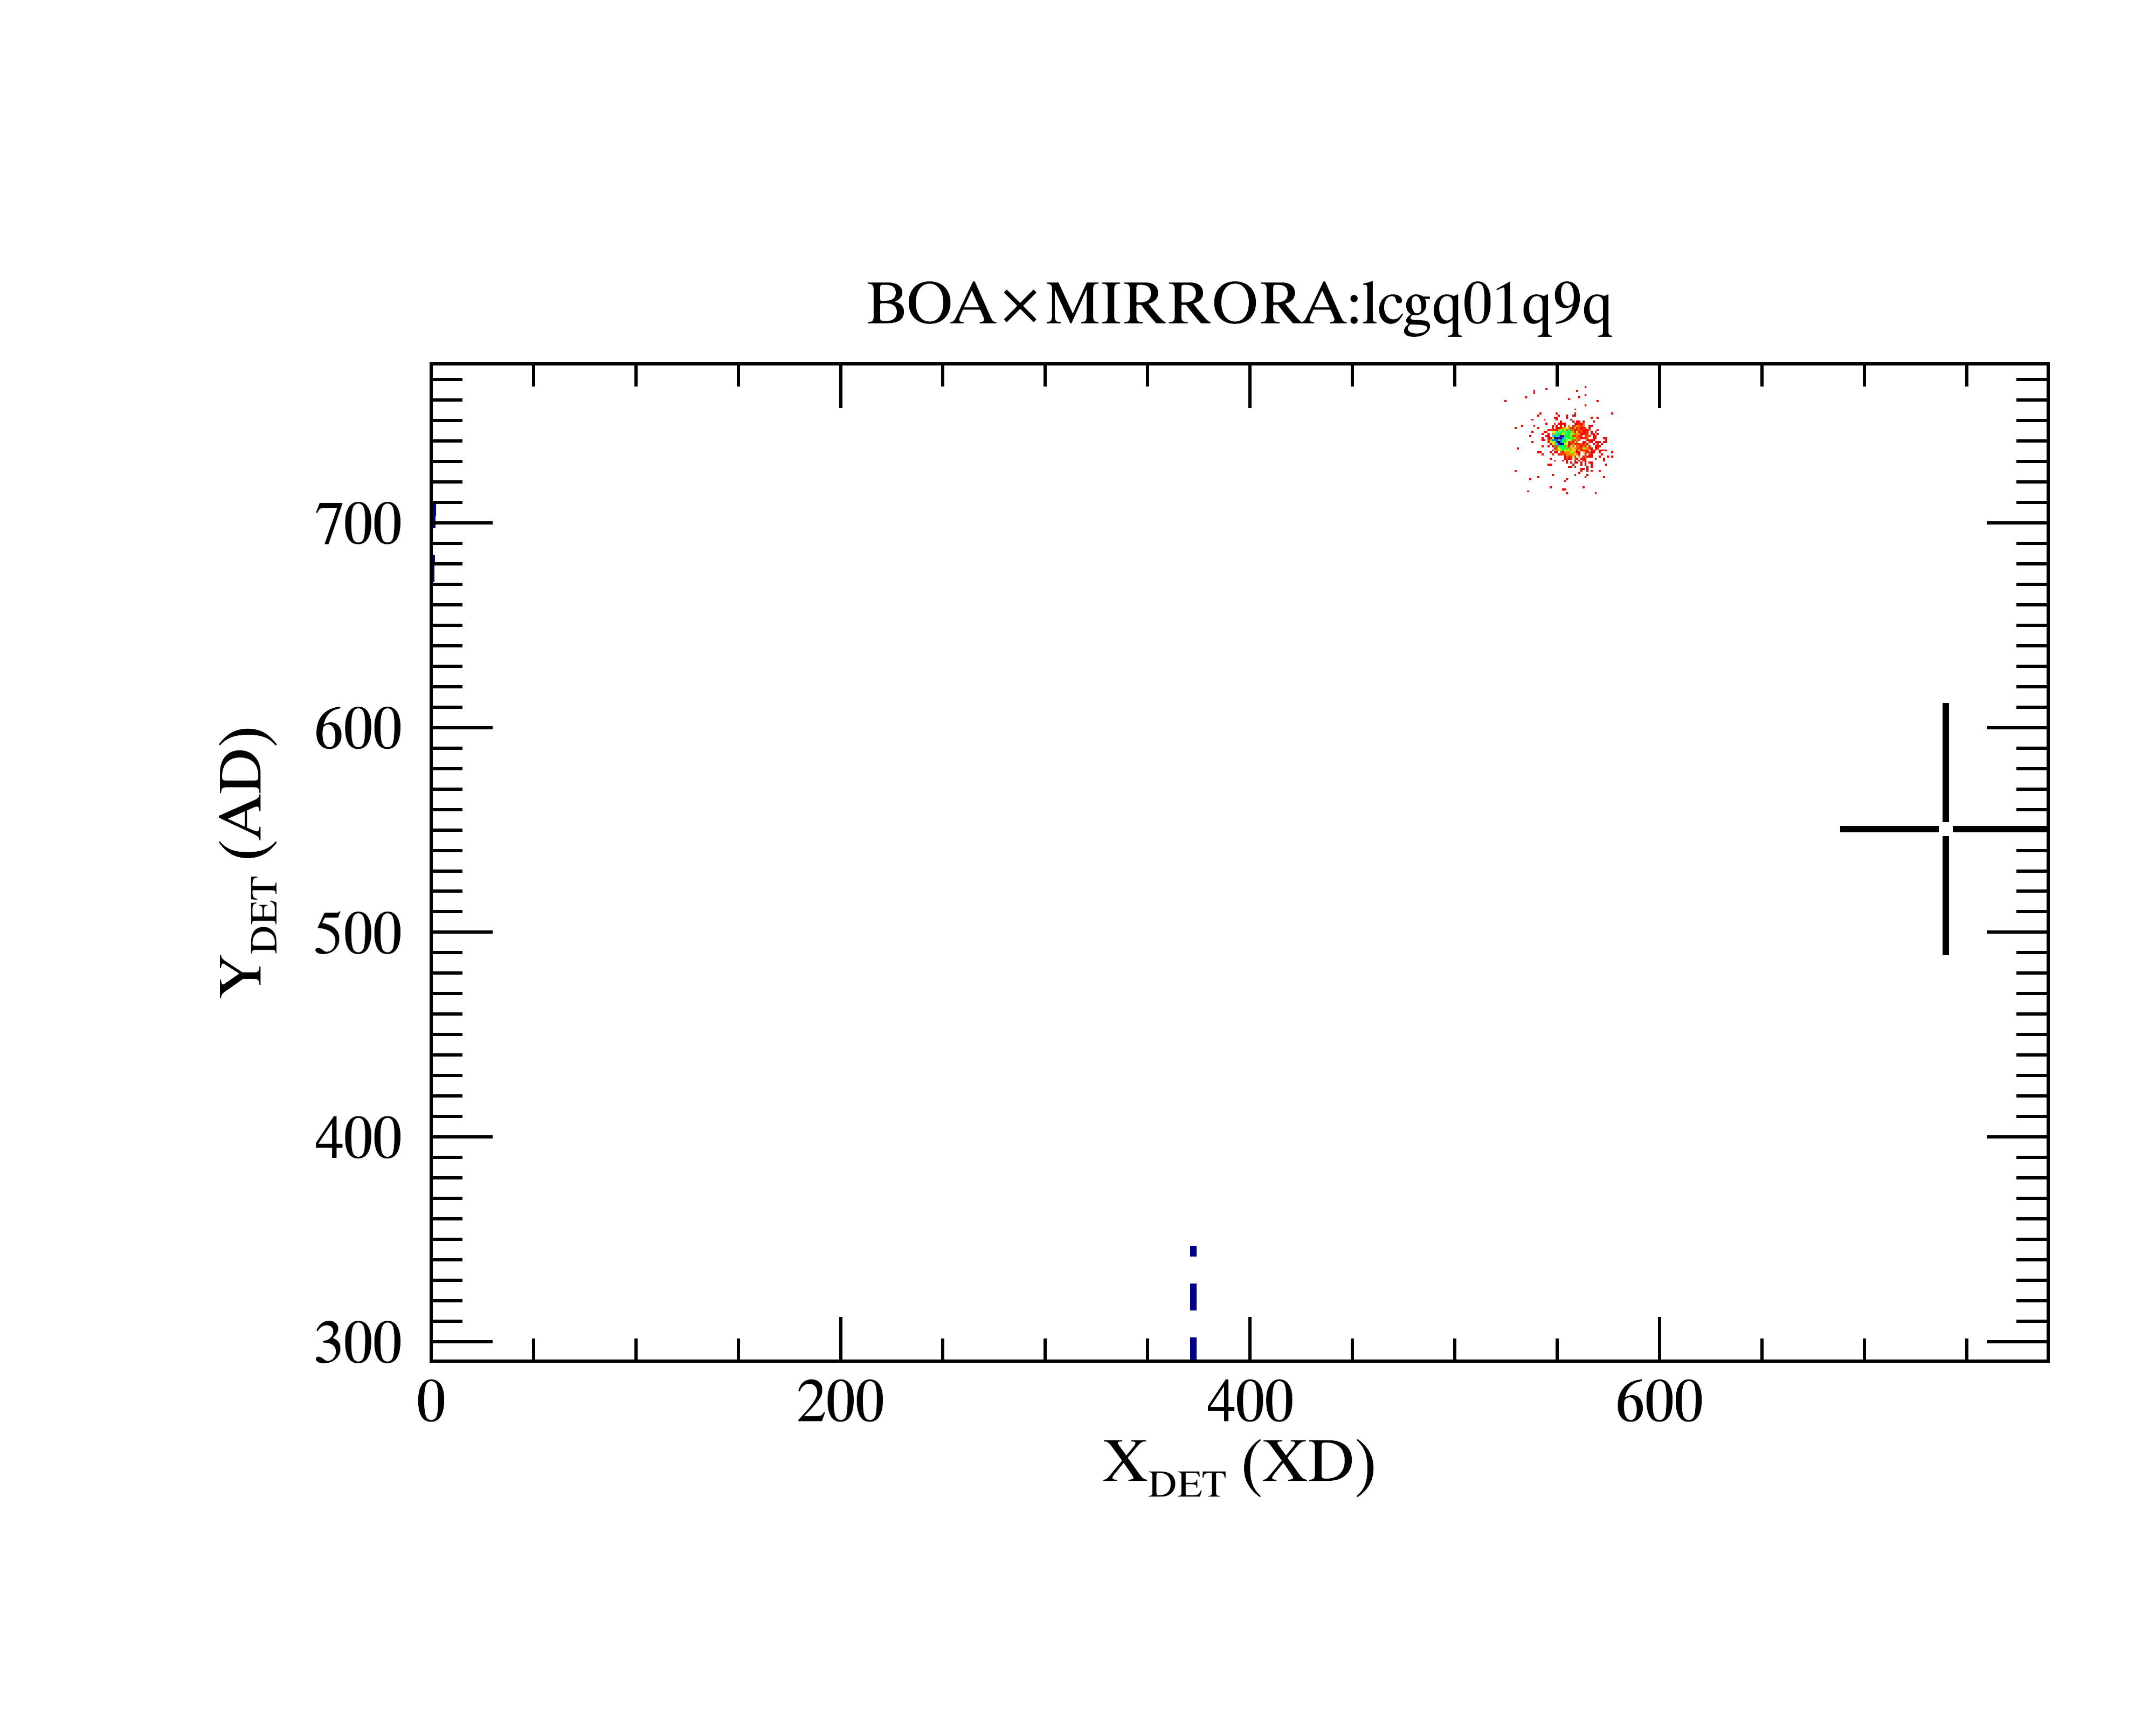
\includegraphics[width=1in]{png/lcgq01q9q_sa.png}}} \\
% &lcgq01q9q & \textit{ROOTNAME} & lcgq01q9q &  \\
% &[479.0,370.0] & [AD,XD] Standard Measurement & [550.3,739.9] &   \\
% &[479.0,368.0] & [AD,XD] Alternate Measurement & [3.6,3.7] & \\
% &[0.0,2.0] & [AD,XD] Standard - Alternate  & [546.7,736.2] & \\
%\bottomrule
%\end{tabular}
%\end{table}
